\begin{textbox}{\href{https://compneuro.neuromatch.io/tutorials/W2D4_DynamicNetworks/chapter_title.html}{Neural Rate Models (W2D4T1)} }
\begin{subbox}{subbox}{Dynamics of a single excitatory population}
\scriptsize
Individual neurons respond by spiking. When we average the spikes of neurons in a population, we can define the average firing activity of the population. In this model, we are interested in how the population-averaged firing varies as a function of time and network parameters. Mathematically, we can describe the firing rate dynamic of a feed-forward network as:
$$ \tau \frac{dr}{dt} &= -r + F(I_{\text{ext}})  \quad $$
$r(t)$ represents the average firing rate of the excitatory population at time $t$, $\tau$ controls the timescale of the evolution of the average firing rate, $I_{\text{ext}}$ represents the external input, and the transfer function $F(\cdot)$ (which can be related to f-I curve of individual neurons described in the next sections) represents the population activation function in response to all received inputs.


\end{subbox}
\begin{subbox}{subbox}{F-I (firing rate vs. input) curve}
\scriptsize
In electrophysiology, a neuron is often characterized by its spike rate output in response to input currents. This is often called the F-I curve, denoting the output spike frequency (F) in response to different injected currents (I). 

The transfer function $F(\cdot)$ in Equation $1$ represents the gain of the population as a function of the total input. The gain is often modeled as a sigmoidal function, i.e., more input drive leads to a nonlinear increase in the population firing rate. The output firing rate will eventually saturate for high input values. 

A sigmoidal $F(\cdot)$ is parameterized by its gain $a$ and threshold $\theta$.
$$ F(x;a,\theta) = \frac{1}{1+\text{e}^{-a(x-\theta)}} - \frac{1}{1+\text{e}^{a\theta}} $$

The argument $x$ represents the input to the population. Note that the second term is chosen so that $F(0;a,\theta)=0$.

\begin{center}
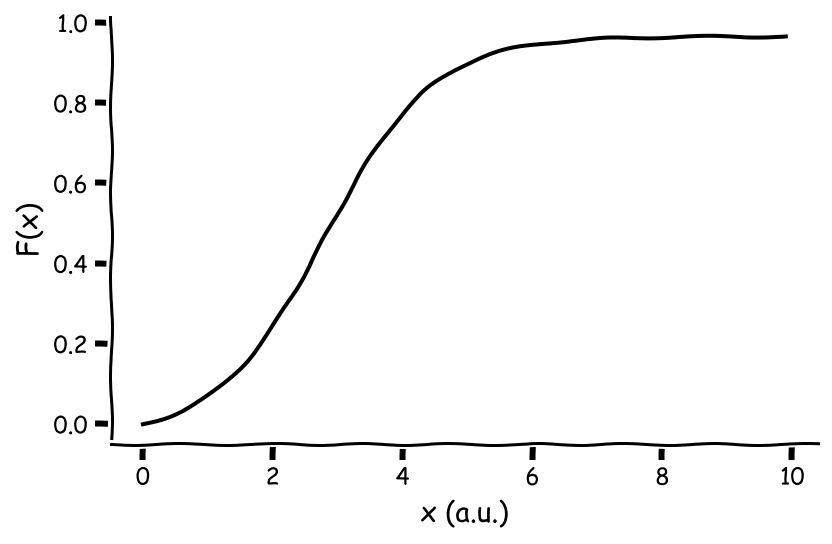
\includegraphics[scale=0.18]{Figures/DN/DN_Figure1.png}
\end{center}
\end{subbox}

\end{textbox}
%%%%%%%%%%%%%%%%%%%%%%%%%%%%%%%%%%%%%%%%%%%%%%%%%%%%%%
%%%%%%%%%%%%%%%%%%%%%%%%%%%%%%%%%%%%%%%%%%%%%%%%%%%%%%
\begin{textbox}{\href{https://compneuro.neuromatch.io/tutorials/W2D4_DynamicNetworks/chapter_title.html}{Neural Rate Models (W2D4T1)} }
\begin{subbox}{subbox}{Fixed points of the single population system}
\scriptsize
We can now extend our feed-forward network to a recurrent network, governed by the equation:

\begin{equation*}
\tau \frac{dr}{dt} &= -r + F(w\cdot r + I_{\text{ext}})  \quad\qquad (+)
\end{equation*}

where as before, $r(t)$ represents the average firing rate of the excitatory population at time $t$, $\tau$ controls the timescale of the evolution of the average firing rate, $I_{\text{ext}}$ represents the external input, and the transfer function $F(\cdot)$ (which can be related to f-I curve of individual neurons described in the next sections) represents the population activation function in response to all received inputs. Now we also have $w$ which denotes the strength (synaptic weight) of the recurrent input to the population.

As you varied the two parameters in the last Interactive Demo, you noticed that, while at first the system output quickly changes, with time, it reaches its maximum/minimum value and does not change anymore. The value eventually reached by the system is called the \textbf{steady state} of the system, or the \textbf{fixed point}. Essentially, in the steady states the derivative with respect to time of the activity ($r$) is zero, i.e. $\displaystyle \frac{dr}{dt}=0$. 

We can find that the steady state of the Equation ($+$) by setting $\displaystyle{\frac{dr}{dt}=0}$ and solve for $r$:
\begin{equation*}
-r_{\text{steady}} + F(w\cdot r_{\text{steady}} + I_{\text{ext}};a,\theta) = 0 \qquad (\ddagger)
\end{equation*}
When it exists, the solution of Equation ($\ddagger$) defines a \textbf{fixed point} of the dynamical system in Equation ($+$). Note that if $F(x)$ is nonlinear, it is not always possible to find an analytical solution, but the solution can be found via numerical simulations.
In the specific case of $w=0$, we can also analytically compute  the solution of Equation ($+$) and deduce the role of $\tau$ in determining the convergence to the fixed point: 
\begin{equation*}
\displaystyle{r(t) = \big{[}F(I_{\text{ext}};a,\theta) -r(t=0)\big{]} (1-\text{e}^{-\frac{t}{\tau}})} + r(t=0)
\end{equation*}
We can now numerically calculate the fixed point with a root finding algorithm.
\begin{center}
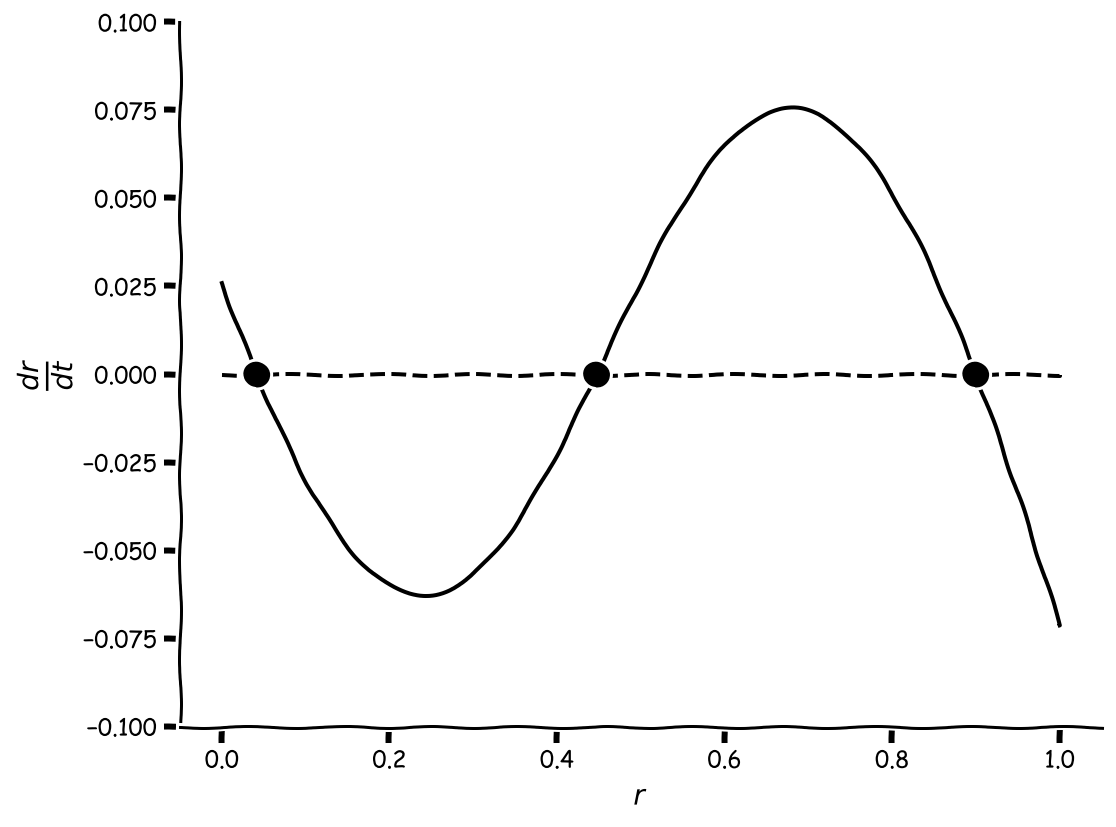
\includegraphics[scale=0.1]{Figures/DN/DN_Figure2.png}
\end{center}
\end{subbox}

\end{textbox}
%%%%%%%%%%%%%%%%%%%%%%%%%%%%%%%%%%%%%%%%%%%%%%%%%%%%%%
%%%%%%%%%%%%%%%%%%%%%%%%%%%%%%%%%%%%%%%%%%%%%%%%%%%%%%
\begin{textbox}{\href{https://compneuro.neuromatch.io/tutorials/W2D4_DynamicNetworks/chapter_title.html}{Neural Rate Models (W2D4T1)} }
\begin{subbox}{subbox}{Fixed points of the single population system}
\scriptsize
Relationship between trajectories & fixed points

Let's examine the relationship between the population activity over time and the fixed points.

Here, let us first set $w=5.0$ and $I_{\text{ext}}=0.5$, and investigate the dynamics of $r(t)$ starting with different initial values $r(0) \equiv r_{\text{init}}$. 


We will plot the trajectories of $r(t)$ with different initial values $r(0) \equiv r_{\text{init}}  = 0.0, 0.1, 0.2,..., 0.9$.
We have three fixed points but only two steady states showing up - what's happening? 

It turns out that the stability of the fixed points matters. If a fixed point is stable, a trajectory starting near that fixed point will stay close to that fixed point and converge to it (the steady state will equal the fixed point). If a fixed point is unstable, any trajectories starting close to it will diverge and go towards stable fixed points. In fact, the only way for a trajectory to reach a stable state at an unstable fixed point is if the initial value \textbf{exactly} equals the value of the fixed point.

We can simulate the trajectory if we start at the unstable fixed point: you can see that it remains at that fixed point (the red line below).

\begin{center}
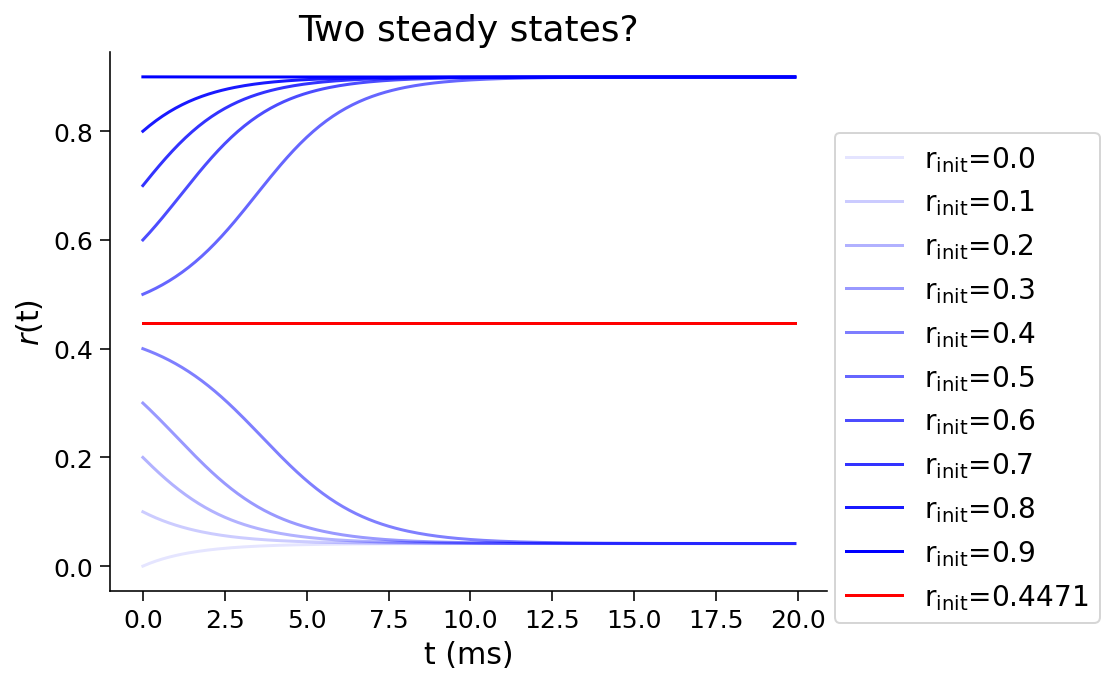
\includegraphics[scale=0.3]{Figures/DN/DN_Figure4.png}
\end{center}
\end{subbox}

\end{textbox}
%%%%%%%%%%%%%%%%%%%%%%%%%%%%%%%%%%%%%%%%%%%%%%%%%%%%%%
%%%%%%%%%%%%%%%%%%%%%%%%%%%%%%%%%%%%%%%%%%%%%%%%%%%%%%
\begin{textbox}{\href{https://compneuro.neuromatch.io/tutorials/W2D4_DynamicNetworks/chapter_title.html}{Wilson-Cowan Model (W2D4T2)} }
\begin{subbox}{subbox}{Mathematical description of the WC model}
\scriptsize
Many of the rich dynamics recorded in the brain are generated by the interaction of excitatory and inhibitory subtype neurons. Here, similar to what we did in the previous tutorial, we will model two coupled populations of E and I neurons (\textbf{Wilson-Cowan} model). We can write two coupled differential equations, each representing the dynamics of the excitatory or inhibitory population:

\begin{align*}
\tau_E \frac{dr_E}{dt} &= -r_E + F_E(w_{EE}r_E -w_{EI}r_I + I^{\text{ext}}_E;a_E,\theta_E)\\
\tau_I \frac{dr_I}{dt} &= -r_I + F_I(w_{IE}r_E -w_{II}r_I + I^{\text{ext}}_I;a_I,\theta_I)    
\end{align*}

$r_E(t)$ represents the average activation (or firing rate) of the excitatory population at time $t$, and $r_I(t)$ the activation (or firing rate) of the inhibitory population. The parameters $\tau_E$ and $\tau_I$ control the timescales of the dynamics of each population. Connection strengths are given by: $w_{EE}$ (E $\rightarrow$ E), $w_{EI}$ (I $\rightarrow$ E), $w_{IE}$ (E $\rightarrow$ I), and $w_{II}$ (I $\rightarrow$ I). The terms $w_{EI}$ and $w_{IE}$ represent connections from inhibitory to excitatory population and vice versa, respectively. The transfer functions (or F-I curves) $F_E(x;a_E,\theta_E)$ and $F_I(x;a_I,\theta_I)$ can be different for the excitatory and the inhibitory populations.
\begin{center}
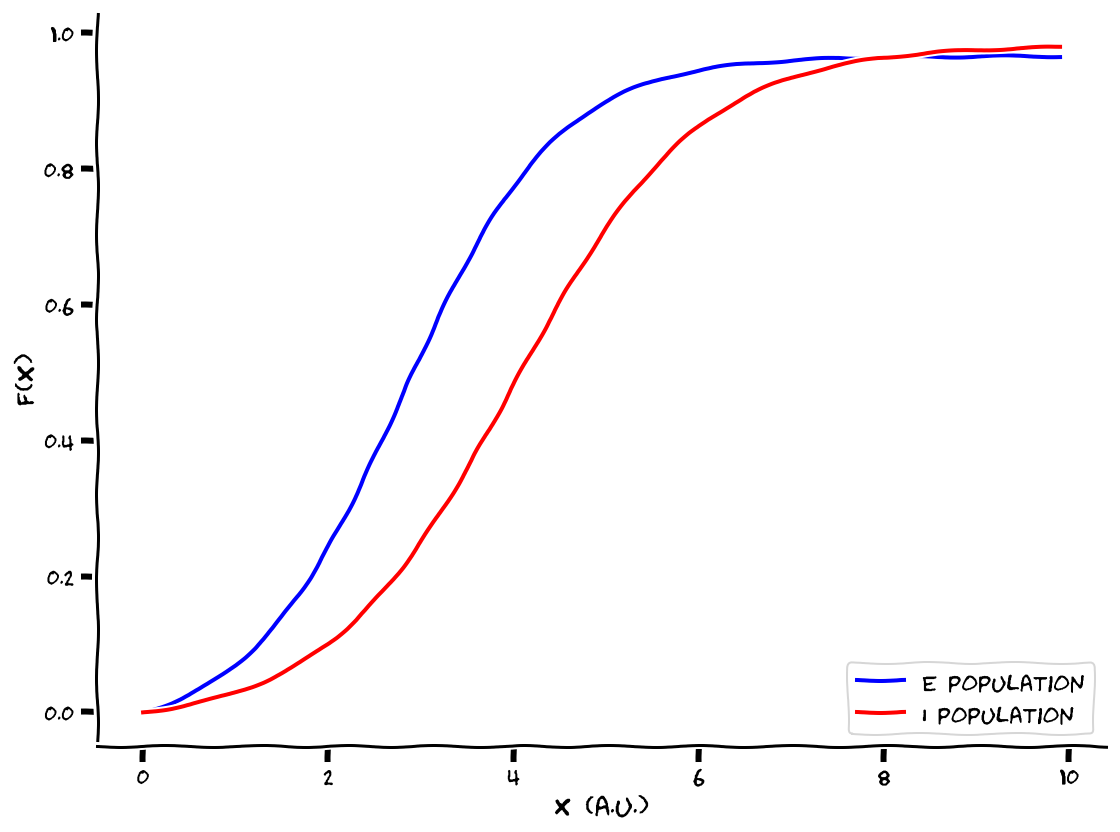
\includegraphics[scale=0.28]{Figures/DN/DN_Figure5.png}
\end{center}
\end{subbox}

\end{textbox}
%%%%%%%%%%%%%%%%%%%%%%%%%%%%%%%%%%%%%%%%%%%%%%%%%%%%%%
%%%%%%%%%%%%%%%%%%%%%%%%%%%%%%%%%%%%%%%%%%%%%%%%%%%%%%
\begin{textbox}{\href{https://compneuro.neuromatch.io/tutorials/W2D4_DynamicNetworks/chapter_title.html}{Wilson-Cowan Model (W2D4T2)} }
\begin{subbox}{subbox}{Numerically integrate the Wilson-Cowan equations}
\scriptsize

Once again, we can integrate our equations numerically. Using the Euler method, the dynamics of E and I populations can be simulated on a time-grid of stepsize $\Delta t$. The updates for the activity of the excitatory and the inhibitory populations can be written as:

\begin{align*}
r_E[k+1] &= r_E[k] + \Delta r_E[k]\\
r_I[k+1] &= r_I[k] + \Delta r_I[k] 
\end{align*}

with the increments

\begin{align*}
\Delta r_E[k] &= \frac{\Delta t}{\tau_E}[-r_E[k] + F_E(w_{EE}r_E[k] \\
&-w_{EI}r_I[k] + I^{\text{ext}}_E[k];a_E,\theta_E)]\\
\Delta r_I[k] &= \frac{\Delta t}{\tau_I}[-r_I[k] + F_I(w_{IE}r_E[k] \\
&-w_{II}r_I[k] + I^{\text{ext}}_I[k];a_I,\theta_I)] 
\end{align*}

The two plots above show the temporal evolution of excitatory ($r_E$, blue) and inhibitory ($r_I$, red) activity for two different sets of initial conditions.

\begin{center}
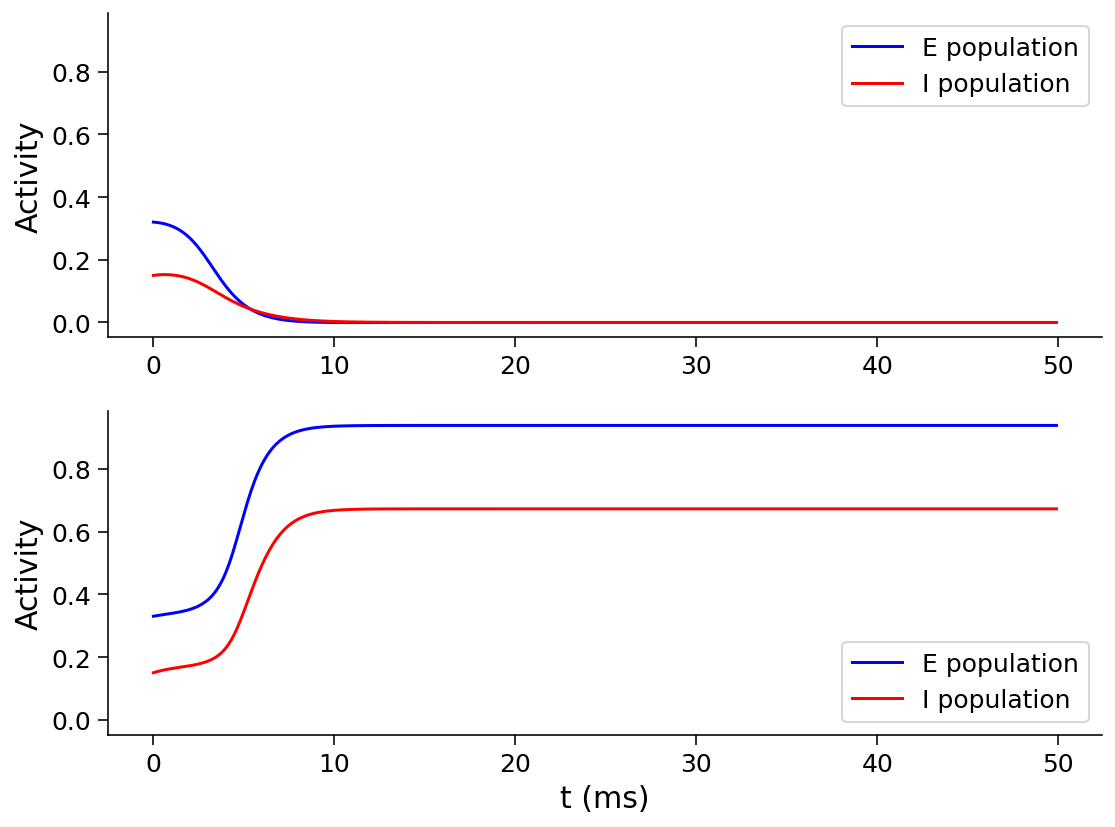
\includegraphics[scale=0.3]{Figures/DN/DN_Figure6.png}
\end{center}
\end{subbox}

\end{textbox}
%%%%%%%%%%%%%%%%%%%%%%%%%%%%%%%%%%%%%%%%%%%%%%%%%%%%%%
%%%%%%%%%%%%%%%%%%%%%%%%%%%%%%%%%%%%%%%%%%%%%%%%%%%%%%
\begin{textbox}{\href{https://compneuro.neuromatch.io/tutorials/W2D4_DynamicNetworks/chapter_title.html}{Wilson-Cowan Model (W2D4T2)} }
\begin{subbox}{subbox}{Phase plane analysis}
\scriptsize
Just like we used a graphical method to study the dynamics of a 1-D system in the previous tutorial, here we will learn a  graphical approach called \textbf{phase plane analysis} to study the dynamics of a 2-D system like the Wilson-Cowan model.

So far, we have plotted the activities of the two populations as a function of time. Instead, we can plot the two activities $r_E(t)$ and $r_I(t)$ against each other at any time point $t$. This characterization in the `rI-rE` plane $(r_I(t), r_E(t))$ is called the \textbf{phase plane}. Each line in the phase plane indicates how both $r_E$ and $r_I$ evolve with time.
\begin{center}
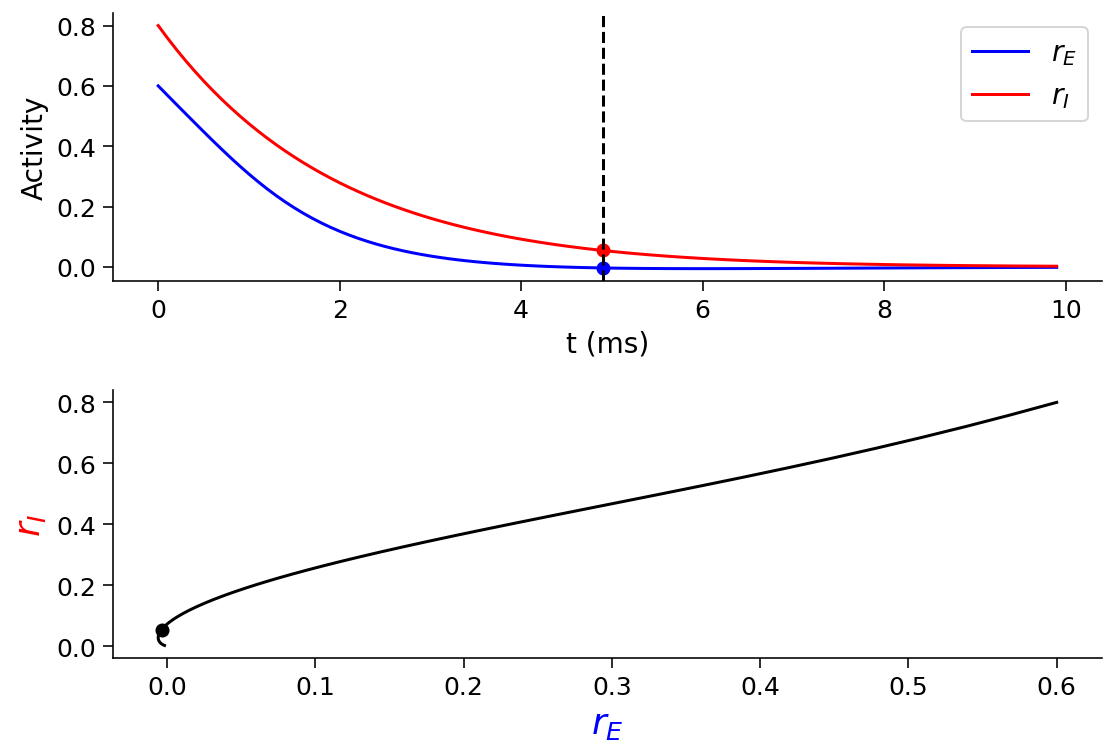
\includegraphics[scale=0.3]{Figures/DN/DN_Figure7.png}
\end{center}
\end{subbox}
\begin{subbox}{subbox}{Nullclines of the Wilson-Cowan Equations
}
\scriptsize
An important concept in the phase plane analysis is the "nullcline" which is defined as the set of points in the phase plane where the activity of one population (but not necessarily the other) does not change.

In other words, the $E$ and $I$ nullclines of Equation $(1)$ are defined as the points where $\displaystyle{\frac{dr_E}{dt}}=0$, for the excitatory nullcline, or $\displaystyle\frac{dr_I}{dt}=0$ for the inhibitory nullcline. That is:

\begin{align*}
-r_E + F_E(w_{EE}r_E -w_{EI}r_I + I^{\text{ext}}_E;a_E,\theta_E) &= 0  \\
-r_I + F_I(w_{IE}r_E -w_{II}r_I + I^{\text{ext}}_I;a_I,\theta_I) &= 0  
\end{align*}
\end{subbox}

\end{textbox}
%%%%%%%%%%%%%%%%%%%%%%%%%%%%%%%%%%%%%%%%%%%%%%%%%%%%%%
%%%%%%%%%%%%%%%%%%%%%%%%%%%%%%%%%%%%%%%%%%%%%%%%%%%%%%
\begin{textbox}{\href{https://compneuro.neuromatch.io/tutorials/W2D4_DynamicNetworks/chapter_title.html}{Wilson-Cowan Model (W2D4T2)} }

\begin{subbox}{subbox}{Compute the nullclines of the Wilson-Cowan model}
\scriptsize
Along the nullcline of excitatory population , you can calculate the inhibitory activity by rewriting it as 

\begin{align*}
r_I = \frac{1}{w_{EI}}\big{[}w_{EE}r_E - F_E^{-1}(r_E; a_E,\theta_E) + I^{\text{ext}}_E \big{]}.
\end{align*}

where $F_E^{-1}(r_E; a_E,\theta_E)$ is the inverse of the excitatory transfer function (defined below). 

Along the nullcline of inhibitory population, you can calculate the excitatory activity by rewriting it as  
\begin{align*}
r_E = \frac{1}{w_{IE}} \big{[} w_{II}r_I + F_I^{-1}(r_I;a_I,\theta_I) - I^{\text{ext}}_I \big{]}  
\end{align*}

where $F_I^{-1}(r_I; a_I,\theta_I)$ is the inverse of the inhibitory transfer function.

The inverse of the sigmoid shaped **f-I** function that we have been using is:

$$
F^{-1}(x; a, \theta) = -\frac{1}{a} \ln \left[ \frac{1}{x + \displaystyle \frac{1}{1+\text{e}^{a\theta}}} - 1 \right] + \theta.
$$
\begin{center}
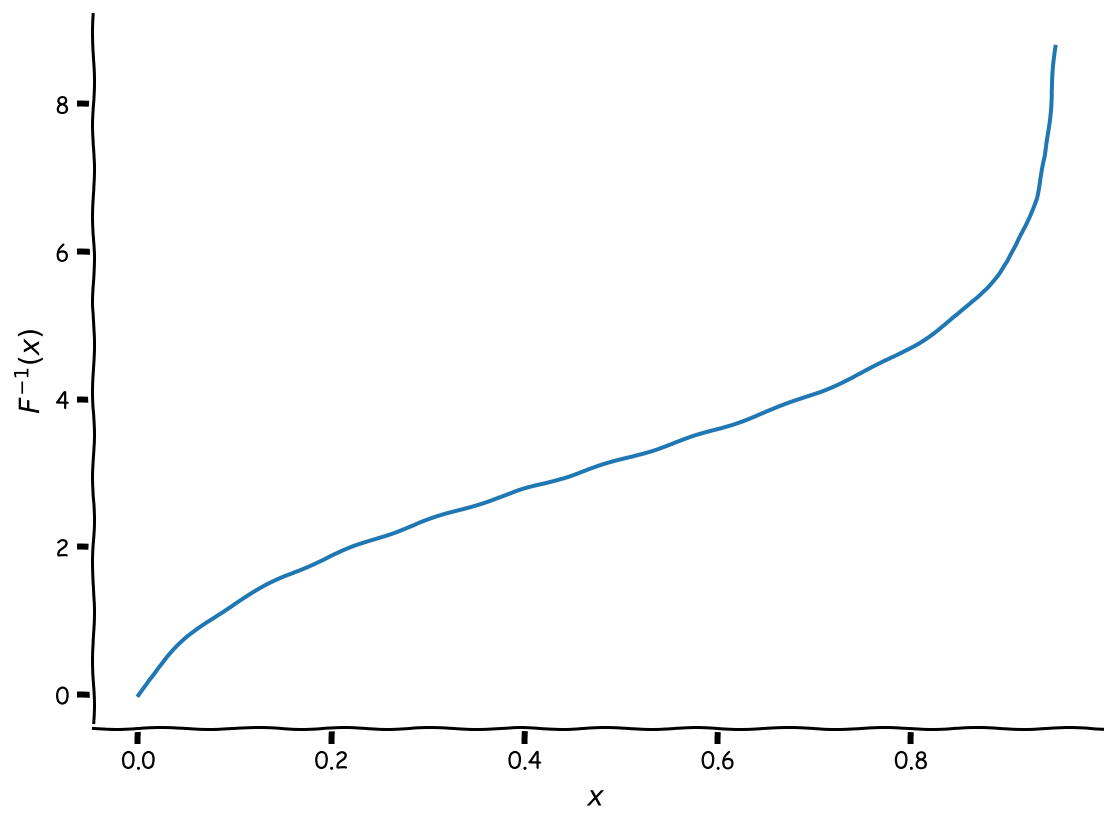
\includegraphics[scale=0.15]{Figures/DN/DN_Figure8.png}
\end{center}
Now you can plot the nullclines
\begin{center}
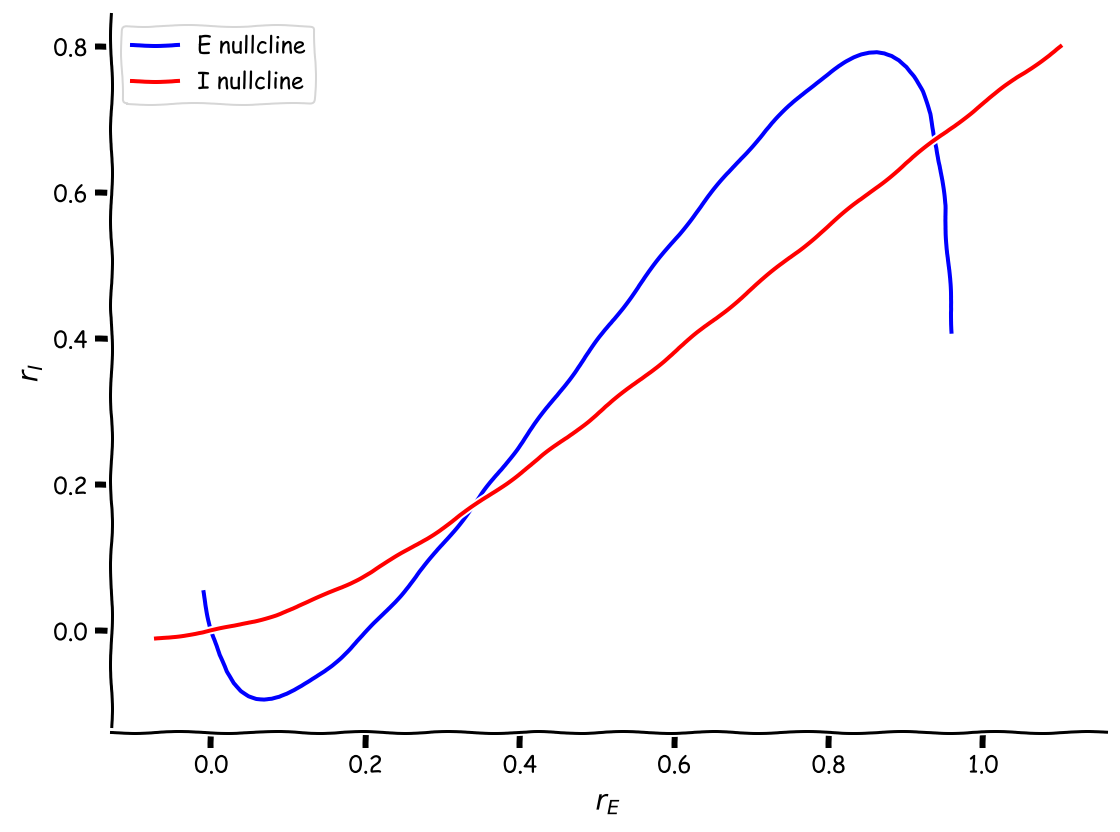
\includegraphics[scale=0.15]{Figures/DN/DN_Figure9.png}
\end{center}

\end{subbox}
\end{textbox}
%%%%%%%%%%%%%%%%%%%%%%%%%%%%%%%%%%%%%%%%%%%%%%%%%%%%%%
%%%%%%%%%%%%%%%%%%%%%%%%%%%%%%%%%%%%%%%%%%%%%%%%%%%%%%
\begin{textbox}{\href{https://compneuro.neuromatch.io/tutorials/W2D4_DynamicNetworks/chapter_title.html}{Wilson-Cowan Model (W2D4T2)} }

\begin{subbox}{subbox}{Vector field}
\scriptsize
How can the phase plane and the nullcline curves help us understand the behavior of the Wilson-Cowan model?

The activities of the $E$ and $I$ populations $r_E(t)$ and $r_I(t)$ at each time point $t$ correspond to a single point in the phase plane, with coordinates $(r_E(t),r_I(t))$. Therefore, the time-dependent trajectory of the system can be described as a continuous curve in the phase plane, and the tangent vector to the trajectory, which is defined as the vector $\bigg{(}\displaystyle{\frac{dr_E(t)}{dt},\frac{dr_I(t)}{dt}}\bigg{)}$, indicates the direction towards which the activity is evolving and how fast is the activity changing along each axis. In fact, for each point $(E,I)$ in the phase plane, we can compute the tangent vector $\bigg{(}\displaystyle{\frac{dr_E}{dt},\frac{dr_I}{dt}}\bigg{)}$, which  indicates the behavior of the system when it traverses that point. 

The map of tangent vectors in the phase plane is called \textbf{vector field}. The behavior of any trajectory in the phase plane is determined by \begin{enumerate}
    \item 
the initial conditions $(r_E(0),r_I(0))$, and 
\item the vector field $\bigg{(}\displaystyle{\frac{dr_E(t)}{dt},\frac{dr_I(t)}{dt}}\bigg{)}$.
\end{enumerate} 
In general, the value of the vector field at a particular point in the phase plane is represented by an arrow. The orientation and the size of the arrow reflect the direction and the norm of the vector, respectively.

To compute and plot the vector field we use
\begin{align*}
\frac{dr_E}{dt} &= [-r_E + F_E(w_{EE}r_E -w_{EI}r_I + I^{\text{ext}}_E;a_E,\theta_E)]\frac{1}{\tau_E}\\
\frac{dr_I}{dt} &= [-r_I + F_I(w_{IE}r_E -w_{II}r_I + I^{\text{ext}}_I;a_I,\theta_I)]\frac{1}{\tau_I}.   
\end{align*}

The phase plane plot below shows us that:

\begin{itemize}
    \item 
 Trajectories seem to follow the direction of the vector field.
\item Different trajectories eventually always reach one of two points depending on the initial conditions.
\item The two points where the trajectories converge are the intersection of the two nullcline curves.
\end{itemize}


\begin{center}
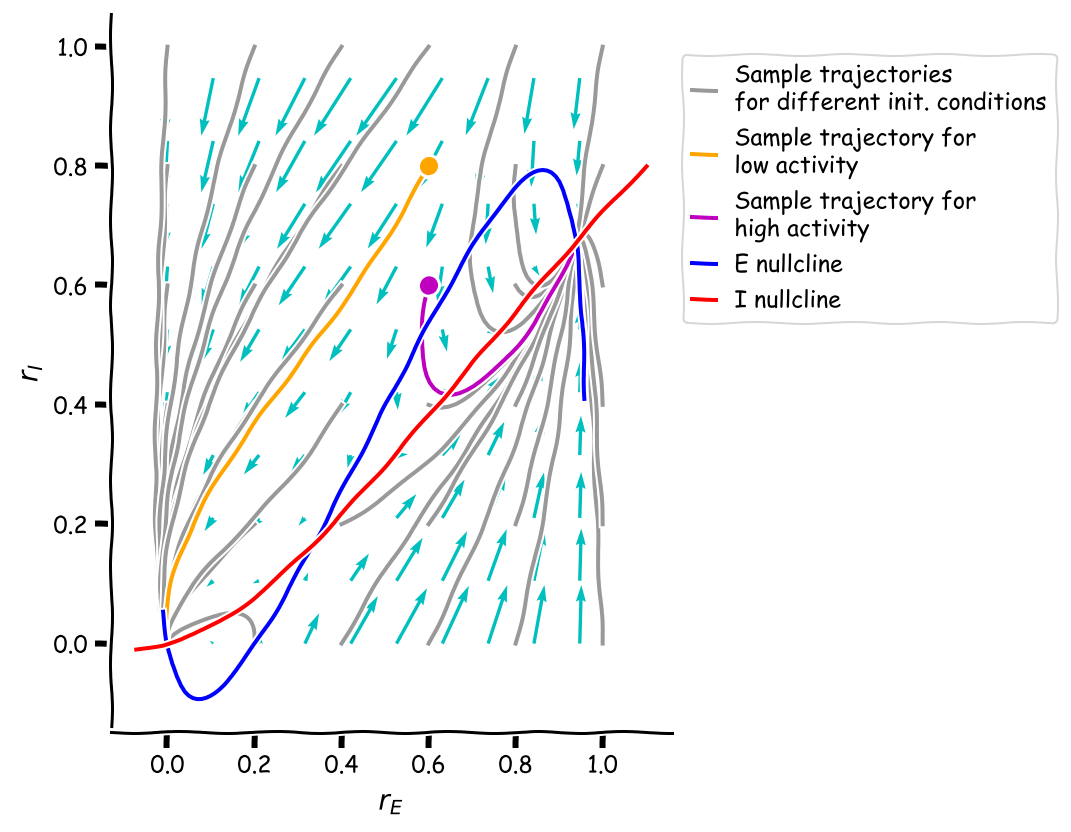
\includegraphics[scale=0.15]{Figures/DN/DN_Figure10.png}
\end{center}

\end{subbox}
\end{textbox}